\documentclass[../sparc.tex]{subfiles}
\graphicspath{{\subfix{../images/}}}
\begin{document}

%%%%%%%%%%%%%%%%%%%%%%%%%%%%%%%%%%%%%%%%%%%%%%%%%%%%%%%%%%%%%%%%%%%%%%%%%%%%%%%%
\section{Работа с макетной платой}

Макетная плата позволяет собирать схемы (подключать электронику) без применения
пайки --- это упрощает прототипирование и ускоряет процесс разработки проектов.
Компоненты просто вставляются в слоты на макетной плате для соединения
(см. рис. \ref{fig:breadboard-led}.)

\begin{figure}[ht]
  \centering
  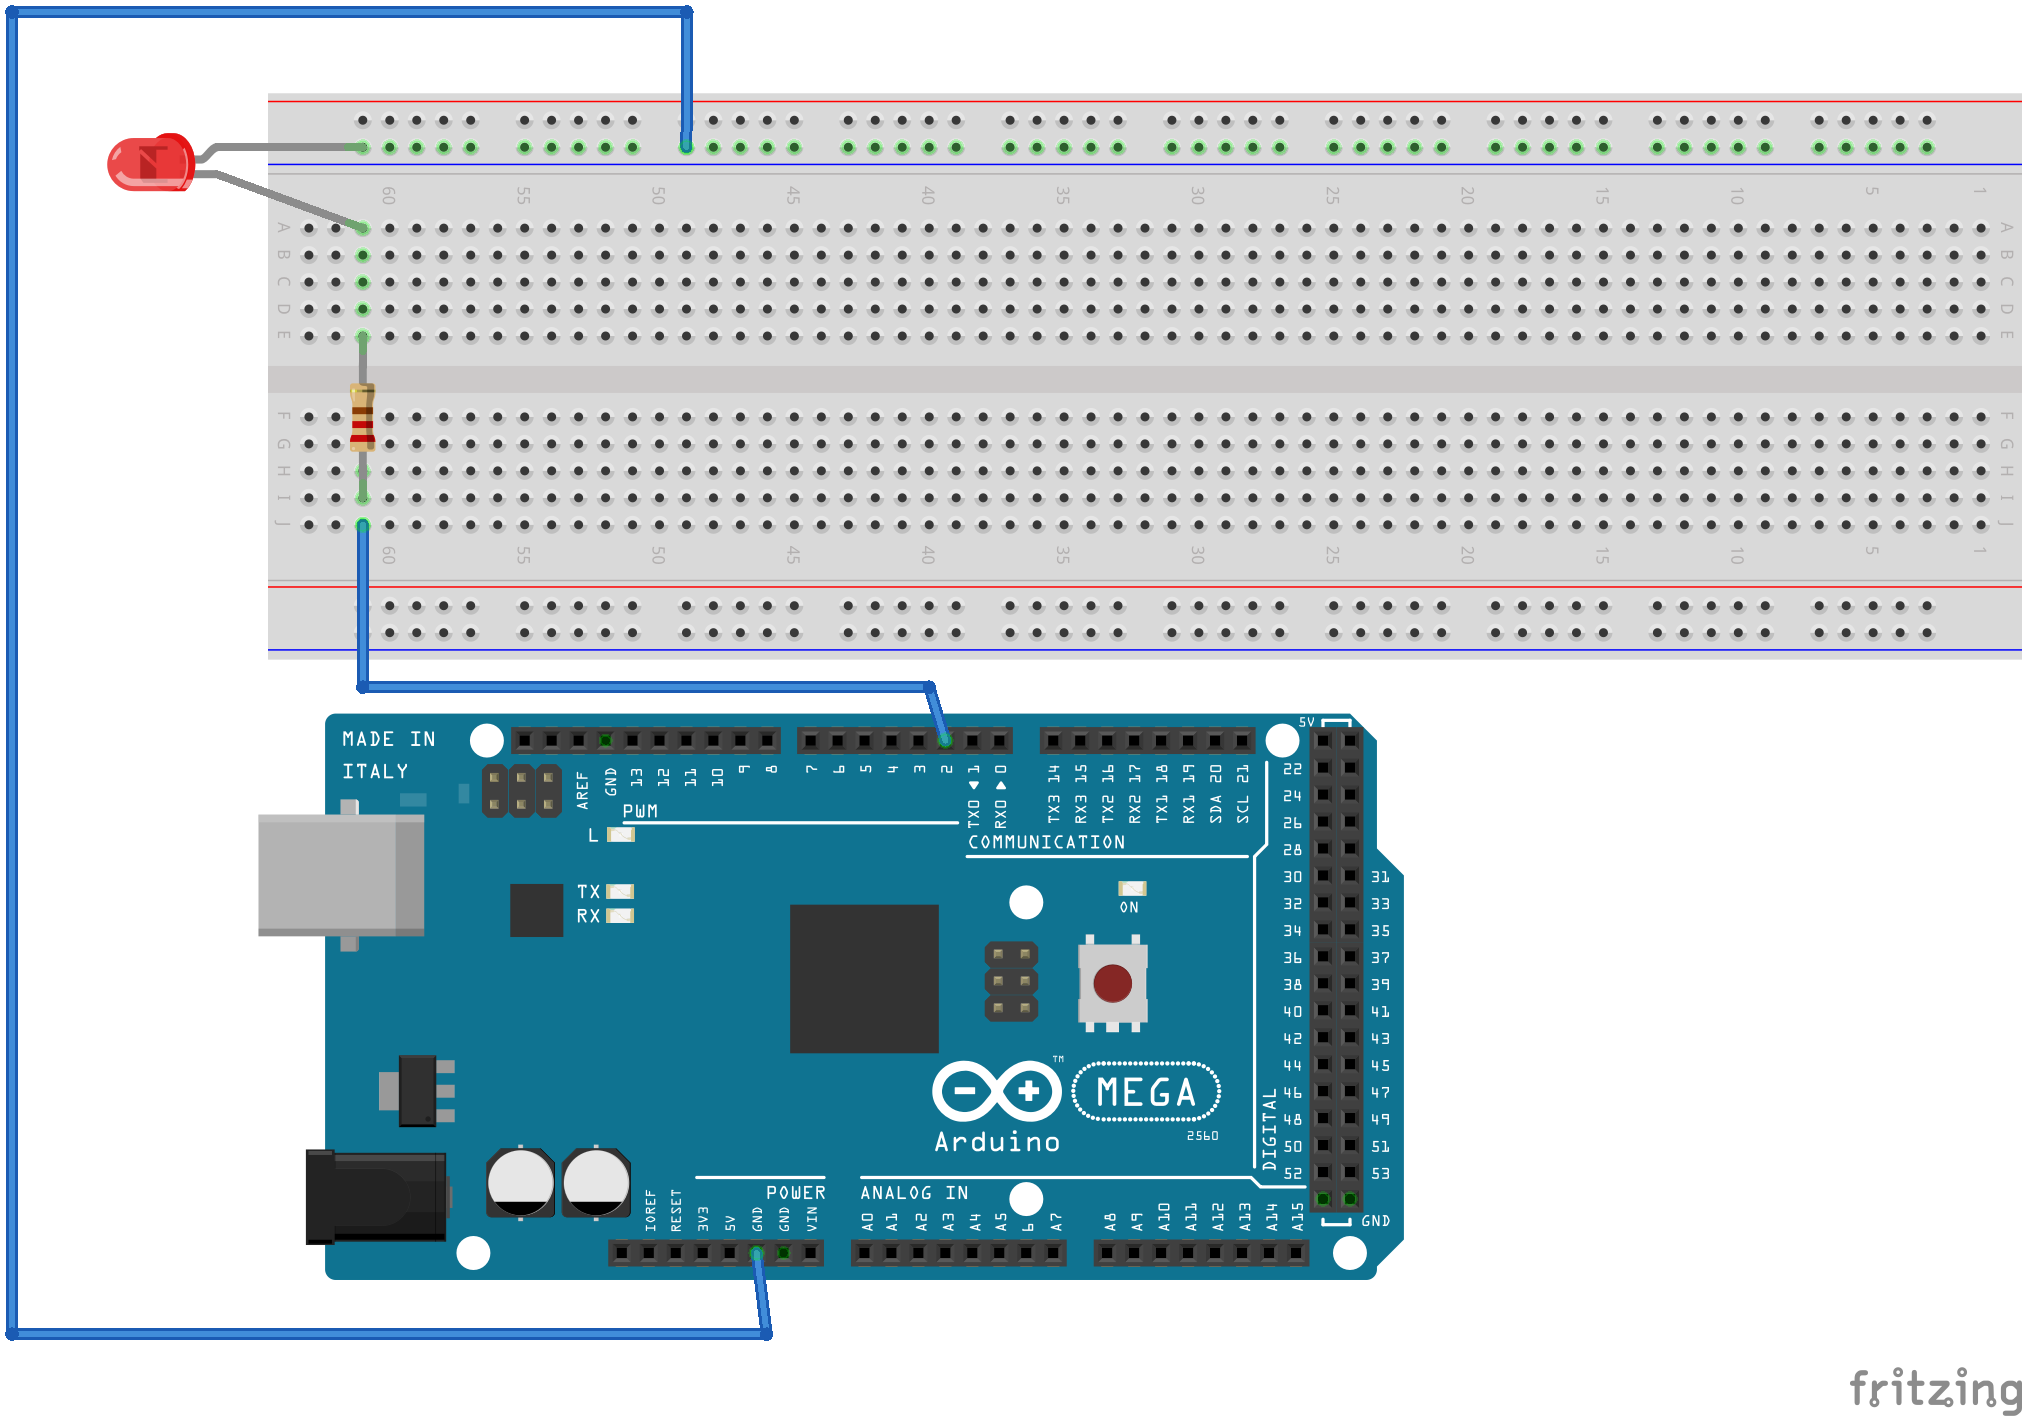
\includegraphics[width=12cm]{schematics/001-led}
  \caption{Пример подключения светодиода на цифровой порт Arduino Mega 2560
    через макетную плату.}
  \label{fig:breadboard-led}
\end{figure}

\begin{itemize}
\item Черный провод подключает минусовой контакт светодиода (катода) на вывод
  ``GND'' Arduino.
\item Синий провод подключает плюсовой контакт светодиода (анод) через резистор
  на цифровой порт номер 2 на Arduino.
\end{itemize}

\note{ Обратите внимание, что светодиоды (и некоторые другие элементы)
  подключаются к платформе Arduino через резистор --- как было сказано в разделе
  \ref{section:electronics-resistance}, резистор позволяет ограничивать ток в
  цепи, тем самым защищая электронные компоненты от преждевременного выхода из
  строя. }

В примере на рис. \ref{fig:breadboard-led} светодиод включится только тогда,
когда на цифровом порту 2 будет достаточное напряжение.  Изначально же на
цифровом порту будет 0 Вольт, и поскольку нет разности потециалов между цифровым
портом и \texttt{GND}, то электрический ток идти не будет.

Таким образом, чтобы зажечь светодиод, мы должны подключить плату Arduino нашей
схемой к компьютеру, написать программу и загрузить её в Arduino.  Все эти этапы
мы рассмотрим в последующих разделах.

%%%%%%%%%%%%%%%%%%%%%%%%%%%%%%%%%%%%%%%%%%%%%%%%%%%%%%%%%%%%%%%%%%%%%%%%%%%%%%%%
\section{Подключение Arduino к компьютеру}
Чтобы подключить Arduino к компьютеру вам потребуется сама платформа Ardu\-ino
(в нашем случае мы используем Arduino Mega 2560) и кабель стандарта USB-В.

Соедините Arduino с компьютером через USB-кабель. Вы увидите, как на плате
загорится светодиод ``ON''.

Теперь необходимо настроить Arduino IDE для работы с подключенной Ardu\-ino, для
этого нужно войти в панель ``Инструменты'' затем ``Плата'' -- в этом меню
необходимо выбрать вариант Arduino, с которой вы сейчас работаете, затем в
подменю ``Порт'' небходимо выбрать порт, к которому подключена Arduino.

\end{document}
